In this chapter we discuss the implementation of the LSTM models described in Chapter 
\ref{lstm theory} and how the predictions of these models are used to try and gain 
insight into what physical processes our models deem the most important.
\section{CamelsML}
Originally a fork of the code in \citet{lstm_second_paper} with a few modifications, 
the machine learning code of this thesis is now implemented to be a fully fledged 
Python package. As the original code it is forked from, it is released under the 
Apache 2.0 license and anyone is therefore free to modify and implement the code 
into their own experiments in the future.
We dub this package CamelsML (Camels Machine Learning).


See Appendix \ref{camelsml documentation} for documentation on how to use the python 
package as well as a minimal running example.

\section{Data split}
With 671 basins in the CAMELS-GB dataset, we run into an issue with perhaps not 
having enough data. This is not a problem for the time series, as they have data 
over several years, but it is indeed a problem for the static features of which there 
are only one data point per basin. To improve our statistics we therefore use 
cross validation. All results in this thesis that compare models to each other 
are made from the same 5-fold cross validation split. The test set is separate 
from this and is only used to later show the performance of a selected model.
we have analyzed the results.

\section{Training Algorithm}
\begin{figure}
\centering
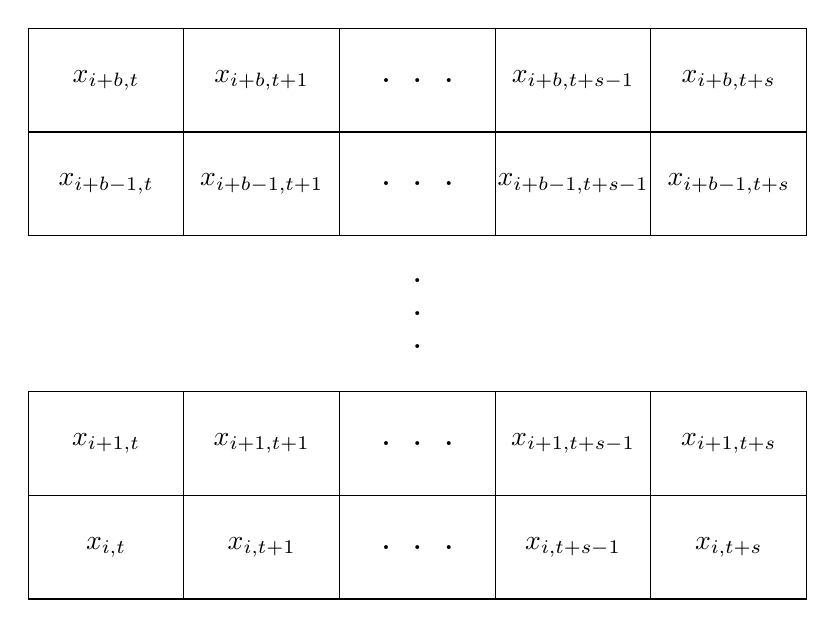
\begin{tikzpicture}[x=0.75pt,y=0.75pt,yscale=-1.25,xscale=1.25]
%uncomment if require: \path (0,300); %set diagram left start at 0, and has height of 300

%Shape: Rectangle [id:dp015989981921256002] 
\draw   (40,200) -- (340,200) -- (340,240) -- (40,240) -- cycle ;
%Shape: Rectangle [id:dp48971481940661865] 
\draw   (40,20) -- (340,20) -- (340,60) -- (40,60) -- cycle ;
%Straight Lines [id:da2960915083454566] 
\draw    (100,20) -- (100,60) ;
%Straight Lines [id:da243954626179525] 
\draw    (160,20) -- (160,60) ;
%Straight Lines [id:da4379878415202513] 
\draw    (220,20) -- (220,60) ;
%Straight Lines [id:da23623272729690736] 
\draw    (280,20) -- (280,60) ;
%Straight Lines [id:da34522789326312586] 
\draw    (100,200) -- (100,240) ;
%Straight Lines [id:da016177459682585327] 
\draw    (220,200) -- (220,240) ;
%Straight Lines [id:da5727133385469978] 
\draw    (280,200) -- (280,240) ;
%Straight Lines [id:da29038977274992184] 
\draw    (160,200) -- (160,240) ;






%Shape: Rectangle [id:dp015989981921256002] 
\draw   (40,160) -- (340,160) -- (340,200) -- (40,200) -- cycle ;
%Shape: Rectangle [id:dp48971481940661865] 
\draw   (40,60) -- (340,60) -- (340,100) -- (40,100) -- cycle ;

%Straight Lines [id:da2960915083454566] 
\draw    (100,60) -- (100,100) ;
%Straight Lines [id:da243954626179525] 
\draw    (160,60) -- (160,100) ;
%Straight Lines [id:da4379878415202513] 
\draw    (220,60) -- (220,100) ;
%Straight Lines [id:da23623272729690736] 
\draw    (280,60) -- (280,100) ;
%Straight Lines [id:da34522789326312586] 
\draw    (100,160) -- (100,200) ;
%Straight Lines [id:da016177459682585327] 
\draw    (220,160) -- (220,200) ;
%Straight Lines [id:da5727133385469978] 
\draw    (280,160) -- (280,200) ;
%Straight Lines [id:da29038977274992184] 
\draw    (160,160) -- (160,200) ;


% Text Node
\draw (190,40) node [anchor=center][inner sep=0.75pt]   [align=left] {{\LARGE . . .}};
% Text Node
\draw (190,220) node [anchor=center][inner sep=0.75pt]   [align=left] {{\LARGE . . .}};
% Text Node
\draw (190,130) node [anchor=center][inner sep=0.75pt]   [align=left] {{\LARGE .}\\{\LARGE .}\\{\LARGE .}};
% Text Node
\draw (70,220) node [anchor=center][inner sep=0.75pt]   [align=left] {$\bm{x}_{i,t}$};
% Text Node
\draw (70,40) node [anchor=center][inner sep=0.75pt]   [align=left] {$\bm{x}_{i+b,t}$};
% Text Node
\draw (130,220) node [anchor=center][inner sep=0.75pt]   [align=left] {$\bm{x}_{i,t+1}$};
% Text Node
\draw (130,40) node [anchor=center][inner sep=0.75pt]   [align=left] {$\bm{x}_{i+b,t+1}$};
% Text Node
\draw (250,40) node [anchor=center][inner sep=0.75pt]   [align=left] {$\bm{x}_{i+b,t+s-1}$};
% Text Node
\draw (250,220) node [anchor=center][inner sep=0.75pt]   [align=left] {$\bm{x}_{i,t+s-1}$};
% Text Node
\draw (310,40) node [anchor=center][inner sep=0.75pt]   [align=left] {$\bm{x}_{i+b,t+s}$};
% Text Node
\draw (310,220) node [anchor=center][inner sep=0.75pt]   [align=left] {$\bm{x}_{i,t+s}$};



\draw (190,80) node [anchor=center][inner sep=0.75pt]   [align=left] {{\LARGE . . .}};
% Text Node
\draw (190,180) node [anchor=center][inner sep=0.75pt]   [align=left] {{\LARGE . . .}};

\draw (70,180) node [anchor=center][inner sep=0.75pt]   [align=left] {$\bm{x}_{i+1,t}$};
% Text Node
\draw (70,80) node [anchor=center][inner sep=0.75pt]   [align=left] {$\bm{x}_{i+b-1,t}$};
% Text Node
\draw (130,180) node [anchor=center][inner sep=0.75pt]   [align=left] {$\bm{x}_{i+1,t+1}$};
% Text Node
\draw (130,80) node [anchor=center][inner sep=0.75pt]   [align=left] {$\bm{x}_{i+b-1,t+1}$};


% Text Node
\draw (250,80) node [anchor=center][inner sep=0.75pt]   [align=left] {$\bm{x}_{i+b-1,t+s-1}$};
% Text Node
\draw (250,180) node [anchor=center][inner sep=0.75pt]   [align=left] {$\bm{x}_{i+1,t+s-1}$};
% Text Node
\draw (310,80) node [anchor=center][inner sep=0.75pt]   [align=left] {$\bm{x}_{i+b-1,t+s}$};
% Text Node
\draw (310,180) node [anchor=center][inner sep=0.75pt]   [align=left] {$\bm{x}_{i+1,t+s}$};
\end{tikzpicture}

\caption{A minibatch. $\bm{x}_{i,t}$ represents the input parameters $\bm{x}$ at time step $t$ for time series $i \in [0, b]$ where $b$ is the batch size. A minibatch consists of $b \times t$ FP32 numbers.}
\label{minibatch}
\end{figure}
Our training algorithm can be described as:
\begin{enumerate}
    \item Split the basins in the training set into 5 parts. Repeat this 5 times, each time using 4/5 parts for training and 1/5 for validation.\begin{enumerate}
        \item Initialize LSTM model with random weights and zero biases, except for the bias of the forget gate $\bm{b}_f$ which is initialized as 5 to make the initial model either forget or remember idk \citationneeded
        \item Split each training basin's time series into several parts, the length 
            of which are decided by the sequence length variable $s$. A minibatch 
            consists of a batch size $s$ amount of these $s$ long timeseries.
        \item For each minibatch:
        \begin{enumerate}
            \item Use the model to predict the outcomes of each timeseries in the 
                minibatch. This can be done in parallel.
            \item Use the average loss of all predictions in the minibatch to update 
                the model parameters using ADAM (see Section \ref{ADAM}).
        \end{enumerate}
        \item Evaluate on the validation set without updating parameters.
    \end{enumerate}
\end{enumerate}
Evaluating our model is done using the Nash–Sutcliffe model efficiency coefficient (NSE) \citep{NSE}.
This metric is similar to the $R^2$ score, but it is specialized for usage 
on hydrological time series.
It is defined as 
\begin{equation}
    \text{NSE} = 1 - \frac{\sum_{t=0}^T\left( y^t - \hat{y}^t\right)}{\sum_{t=0}^T\left(y^t - \bar{\hat{y}}\right)} \label{NSE}
\end{equation}
As we employ cross validation, we  end up with is 5 different models 
for each training run. These models do not necessarily converge to the same parameters 
as each other, making them potentially quite different from one another. To test the 
actual performance of a model (not just relative to other model configurations) we 
therefore need to train a new model with the same configuration (using the same features, 
hyperparameters, etc.) on the entire, undivided training set and test that model 
on the test set. This test result cannot be used to determine relative performance 
between different model configurations, but it can give an indication of the actual, 
real-world performance of a final selected model. Statistically, this is due to the 
fact that optimizing model configuration using the test set would mean overfitting 
on said test set. See \citet{elemstatlearn} for a more detailed explanation.

For models used to validate transfer learning between Camels and Camels-GB, we 
cross validate on one dataset and use all five models from the cross validation 
to make ensemble predictions on the validation split of the other dataset. This 
way we can get more robust statistics also in these results, as \citet{lstm_second_paper} 
showed that there often is a non trivial performance difference between a single
model and a model ensemble. In our case we assume this effect to be even higher 
because of the nature of training and validating on different datasets.

%\section{Model configuration}
%\begin{figure}
%\caption{Our full model configuration using an EA-LSTM \citep{lstm_second_paper}}.
%\end{figure}
\begin{table}
    \centering
    \begin{tabular}{lll}
        \hline
        Label & jeff & poop \\
        \hline
    \end{tabular}
    \caption{Table containing all models trained in this thesis along with their 
    given labels and configuration. The information contained here together with 
    CamelsML should be enough to easily be able to recreate the results in this thesis.
    The model configuration files are also located on the Github page of this thesis.}
    \label{all models}
\end{table}
The models we apply in this thesis are all variants of the LSTM model described 
in Section \ref{LSTM Theory}. Table \ref{all models} shows all model configurations 
trained to create the results in this thesis. Note that we reimplement the same model 
as \cite{lstm_third_paper}, but we train it ourselves. This is to be able to compare 
this model more accurately to the new models trained by having it train and validate 
using the same cross validation seed.
\section{Hardware}
The models are run on three different hardware configurations. The important difference 
between these hardware configurations is the amount of available VRAM. As LSTM models 
are recurrent neural networks they are not as parallelizable as other machine learning 
models (see (\ref{LSTM})). This means that the only way for us to fully exploit 
an increase in VRAM is to parallelize data-wize. To do this we increase the batch size.
The three hardware configurations are listed as follows \footnote{Note that we only 
state the used graphics card as this is the only important difference, we run no 
calculations on processors and do not use a significant amount of ordinary RAM.}:
\begin{enumerate}
    \item Nvidia GTX 980 ti: This has 6 GB of VRAM, we found a batch size of 1024 
        to be a sweet spot here.
    \item Nvidia GTX 1660 ti: Same as above.
    \item Nvidia Tesla V100 (Provided by Simula's eX3 cluster): This has 32 GB of VRAM, we find a batch size of 4096 
        to be a sweet spot. Anything more leads to a downgrade in speed because 
        of limitations in transferring data from the storage device to the GPU. 
        This is still not ideal and leads to an approximate 30\% utilization of the 
        GPU.
\end{enumerate}
We acknowledge that the inconsistent use of batch sizes across models may somewhat 
impact the model performance, as previously stated in Chapter \ref{stochastic gradient descent}.
However, as long as the amount of minibatches is sufficiently smaller than the number of datapoints we 
still get an acceptable amount of stochasticity in the training process and the batch 
size is usually set as high as possible in most machine learning practices because 
of model speed. Batch size is usually set as high as the hardware supports, as long 
as the total size of training data is $>>$VRAM \citationneeded.
Still, in an ideal situation we would use the same hardware for all training runs, 
but in this case we are limited by queue times on Simula's eX3 cluster in addition 
to the as of Q4 2020 $\rightarrow$ Q2 2021 silicon shortage making the acquisition of 
new graphics cards next to impossible \citep{GPUShortage}.
